\documentclass[twoside]{article}
\input{ISC18-english.sty}

%%%%%%%%%%%%%%%%%%%%%%%%%%%%  Make sure to compile twice for proper cross-references. %%%%%%%%%%%%%%%%%%%%%%%
%%%%%%% For proper display of references, compile the document twice. %%%%%%%%%%%%%%%%%%%%% 
%%%%%%%%%%%%%%% If using TeX Live, compile using pdflatex command %%%%%%%%%%%%%%%%%%%%%%%
\begin{document}
\thispagestyle{empty}
%%%%%%%%%%%%%%%%% Article title header  %%%%%%%%%%%%%%%%%%%%
\fancyhead[LE]{Trees for Longitudinal Zero-Inflated Count Data}
%%%%%%%%%%%%%%%%% Article authors header   %%%%%%%%%%%%%%%%%%%%
\fancyhead[RO]{E. Tabrizi}
\begin{center}
{
\includegraphics [height=25mm, width=150.3mm] {Images/isc18E}} \\
\vspace*{-1.8cm}
%\begin{center}
%\color{blue} 
%{\hspace{0.1cm}\rule{\textwidth}{1mm}}\\
%\end{center}
\vspace*{4cm}
%%%%%%%%%%%%%%%%% Article title  %%%%%%%%%%%%%%%%%%%%
{\Large \bf Mixed-Effects Hurdle Trees for Longitudinal Zero-Inflated Count Data}\\
%%%%%%%%%%%%%%%%% Article authors and affiliations %%%%%%%%%%%%%%%%%%%%
{\bf
Elham Tabrizi  \footnote[1]{{\bf Corresponding Author:} {\tt elham.tabrizi@khu.ac.ir }} \\
Department of Mathematics, Faculty of Mathematical Sciences and Computer, Kharazmi University, Tehran, Iran} \\
\end{center}
\rule{\textwidth}{0.2mm}\\
%%%%%%%%%%%%%%%%% Article abstract  %%%%%%%%%%%%%%%%%%%%
\noindent{\bf Abstract:}\\
Longitudinal count data with excess zeros are common in many applied fields, yet flexible tree-based methods for such data remain scarce. This paper introduces the Penalized Quasi-Likelihood Hurdle Tree (PHT), a novel algorithm that combines regression trees with mixed-effects models to capture nonlinear fixed effects and subject specific correlations in zero-inflated longitudinal counts. The PHT employs a penalized quasi-likelihood approximation, alternating between estimating random effects and updating tree-based fixed effects via weighted pseudo-responses. Simulation studies demonstrate that PHT outperforms standard regression trees, Poisson GLMMs, and hurdle GLMMs in terms of predictive accuracy. An application to a salamander abundance dataset further confirms the practical utility of PHT, revealing key ecological drivers while achieving the lowest out-of-sample prediction error. 
 
\noindent{\bf Keywords:} 
Longitudinal data, Zero-inflated count data, Hurdle model, Mixed-effects model, Regression tree, Penalized quasi-likelihood.\\
\noindent{\bf Mathematics Subject Classification (2010):} $\rm 99X99$, $\rm 99X99$, $\rm 99X99$. \\
\hspace{1cm}\rule{\textwidth}{0.2mm}\\
%%%%%%%%%%%%%%
\section{Introduction}

Longitudinal count data are frequently encountered in various applied fields such as medicine, public health, insurance, and ecology. A prevalent characteristic of such data is the presence of excess zeros (structural and sampling zeros), which violates the standard distributional assumptions of traditional Poisson Mixed-Effects Models \citep{MSN2008}. Ignoring this zero-inflation or zero-alteration often leads to overdispersion, biased parameter estimates, and invalid inferences. 

To address the issue of excess zeros, two-part models, specifically Hurdle models, have been widely adopted. A Hurdle model separates the data-generating process into two distinct components: a binary process that determines whether the response is zero or positive, and a zero-truncated count process that models the positive observations. For longitudinal data, incorporating random effects into both components of the Hurdle model is essential to adequately account for the within-subject correlation stemming from repeated measurements \citep{MinAgresti2005}. 

Traditional Mixed-Effects Hurdle Models typically assume a generalized linear relationship between the predictors and the link functions. However, in many practical scenarios, covariate effects are highly non-linear and involve complex, higher-order interactions that are difficult to specify a priori. Tree-based methods, such as Classification and Regression Trees (CART), offer a flexible, non-parametric alternative capable of capturing these complex structures. In recent years, regression trees have been successfully extended to longitudinal and clustered data. Notable advancements include the RE-EM tree \citep{sela2012re} for continuous responses and Generalized Mixed Effects Regression Trees \citep{HLB17} for non-normal exponential family distributions. Despite these methodological advancements, there remains a significant gap in the literature regarding tree-based approaches tailored for longitudinal zero-inflated or Hurdle count data. Fitting a full exact Marginal Maximum Likelihood  model for a Mixed-Effects Hurdle Tree is computationally prohibitive due to the complex integration over random effects at each node splitting step. 

To bridge this gap, this paper proposes a novel and computationally efficient approach termed the PQL-Hurdle-Tree (PHT). By leveraging the Penalized Quasi-Likelihood (PQL) approximation, the PHT algorithm alternates between estimating random effects via an underlying Generalized Linear Mixed Model and updating the non-linear fixed effects using weighted regression trees on pseudo-responses. This strategy allows for fast convergence and flexible non-linear modeling of both the zero-inflation and positive count processes in longitudinal data.
\section{The Proposed PHT Algorithm}\label{sec:pht}
To model longitudinal count responses with excess zeros and within-subject dependence, we propose the Penalized Quasi-Likelihood Hurdle Tree. The method combines regression trees for modeling nonlinear fixed effects with mixed-effects models for capturing subject-specific variability. Let $Y_{ij}$ denote the count response for subject $i=1,\ldots,N$ at occasion $j=1,\ldots,n_i$. We assume a hurdle data-generating mechanism:
\begin{equation*}
	Y_{ij}
	=
	\begin{cases}
		0, & \text{with probability } \theta_{ij},\\
		Y_{ij}^{+}, & \text{with probability } 1-\theta_{ij},
	\end{cases}
\end{equation*}
where
$
	Y_{ij}^{+}\sim ZTP(\lambda_{ij}),
$
and $ZTP(\lambda)$ denotes the zero-truncated Poisson distribution with probability mass function
\begin{equation*}
	P(Y=y \mid Y>0)
	=
	\frac{e^{-\lambda}\lambda^{y}}
	{y!\left(1-e^{-\lambda}\right)},
	\qquad y=1,2,\ldots   .
\end{equation*}
The two model components are specified as
\begin{align}
	\text{logit}(\theta_{ij})
	&=
	f_0(\mathbf{x}_{ij})
	+
	\mathbf{z}_{ij}^{(0)\top}\mathbf{b}_{i0},
	\\
	\log(\lambda_{ij})
	&=
	f_+(\mathbf{x}_{ij})
	+
	\mathbf{z}_{ij}^{(+)\top}\mathbf{b}_{i+}.
\end{align}
Here, $f_0(\cdot)$ and $f_+(\cdot)$ are unknown nonlinear functions estimated using regression trees. For computational simplicity, we assume
$
	\mathbf{b}_{i0}
	\sim
	N(\mathbf{0},D_0)$ and
	$\mathbf{b}_{i+}
	\sim
	N(\mathbf{0},D_+)$
with independence between the two random-effect vectors.
The PHT algorithm alternates between updating the tree-based fixed effects and the subject-specific random effects through a PQL approximation.
\begin{alg}[PHT Algorithm]
	The algorithm proceeds as follows:

	\textbf{Step 0: Initialization.}
	Set $\mathbf b_{i0}^{(0)}=\mathbf 0$, $\mathbf b_{i+}^{(0)}=\mathbf 0$,
	$D_0^{(0)}=\sigma_0^2I$, and $D_+^{(0)}=\sigma_+^2I$.
	Initialize $\hat\theta_{ij}^{(0)}$ as the overall proportion of zeros and
	$\hat\lambda_{ij}^{(0)}=\max(\bar y_+,0.1)$, where $\bar y_+$ is the mean of positive observations.
	
	\textbf{Step 1: Zero Component.}
	Define $Y_{ij}^{(0)}=I(Y_{ij}=0)$.
	At iteration $r$, compute
	$
	\eta_{ij}^{(0)}
	=
	logit\left({\hat\theta_{ij}^{(r-1)}}\right)$
	and the pseudo-response
	\begin{equation*}
		\tilde y_{ij}^{(0)}
		=
		\eta_{ij}^{(0)}
		+
		\frac
		{Y_{ij}^{(0)}-\hat\theta_{ij}^{(r-1)}}
		{\hat\theta_{ij}^{(r-1)}
			\left(1-\hat\theta_{ij}^{(r-1)}\right)}.
	\end{equation*}
	The working weights are
	$
	w_{ij}^{(0)}
	=
	\hat\theta_{ij}^{(r-1)}
	\left(1-\hat\theta_{ij}^{(r-1)}\right)
	$,
	and
	$
	\tilde y_{ij}^{(0)*}
	=
	\tilde y_{ij}^{(0)}
	-
	\mathbf z_{ij}^{(0)\top}\mathbf b_{i0}^{(r-1)}
	$.
	Fit a weighted regression tree to
	$(\tilde y_{ij}^{(0)*},\mathbf x_{ij})$
	using weights $w_{ij}^{(0)}$ to obtain $\hat f_0^{(r)}(\cdot)$.
	Following \cite{HLB17}, the pseudo-data define a working linear mixed model and the random effects are updated by
	\begin{equation*}
		\hat{\mathbf b}_{i0}^{(r)}
		=
		\hat D_0^{(r-1)}
		\left(
		W_i^{(0)\frac12}Z_i^{(0)}
		\right)^T
		\hat V_{i0}^{(r-1)-1}
		\left[
		W_i^{(0)\frac12}\tilde{\mathbf y}_i^{(0)}
		-
		W_i^{(0)\frac12}\hat f_0^{(r)}(X_i)
		\right],
	\end{equation*}
	where
	\begin{equation*}
		\hat V_{i0}^{(r-1)}
		=
		W_i^{(0)\frac12}
		Z_i^{(0)}
		\hat D_0^{(r-1)}
		Z_i^{(0)T}
		W_i^{(0)\frac12}
		+
		\hat\sigma_0^{2(r-1)}I .
	\end{equation*}
	Update
	\begin{equation*}
		\hat D_0^{(r)}
		=
		\frac{1}{N}
		\sum_{i=1}^{N}
		\left[
		\hat{\mathbf b}_{i0}^{(r)}
		\hat{\mathbf b}_{i0}^{(r)T}
		+
		\hat\Sigma_{i0}^{(r)}
		\right],
	\end{equation*}
	with
	\begin{equation*}
		\hat\Sigma_{i0}^{(r)}
		=
		\hat D_0^{(r-1)}
		-
		\hat D_0^{(r-1)}
		Z_i^{(0)T}
		\hat V_{i0}^{(r-1)-1}
		Z_i^{(0)}
		\hat D_0^{(r-1)} .
	\end{equation*}
	The residual variance is updated by
	\begin{equation*}
		\hat\sigma_0^{2(r)}
		=
		\frac
		{
			\sum_{i=1}^{N}
			\left[
			\mathbf r_{i0}^{T}
			W_i^{(0)}
			\mathbf r_{i0}
			+
			\mathrm{tr}
			\!\left(
			W_i^{(0)}
			Z_i^{(0)}
			\hat\Sigma_{i0}^{(r)}
			Z_i^{(0)T}
			\right)
			\right]
		}
		{\sum_{i=1}^{N}n_i},
	\end{equation*}
	where
	$
	\mathbf r_{i0}
	=
	\tilde{\mathbf y}_i^{(0)}
	-
	\hat f_0^{(r)}(X_i)
	-
	Z_i^{(0)}
	\hat{\mathbf b}_{i0}^{(r)}
	$.
	Finally,
	\begin{equation*}
		\hat\theta_{ij}^{(r)}
		=
		\mathrm{logit}^{-1}
		\left[
		\hat f_0^{(r)}(\mathbf x_{ij})
		+
		\mathbf z_{ij}^{(0)\top}
		\hat{\mathbf b}_{i0}^{(r)}
		\right].
	\end{equation*}
	\textbf{Step 2: Positive Count Component.}
	Retain observations with $Y_{ij}>0$.
	Let
	$
	\mu_{ij}^{+}
	=
	\lambda_{ij}/(1-e^{-\lambda_{ij}})
	$
	and
	$
	\eta_{ij}^{(+)}
	=
	\log(\lambda_{ij})
	$.
	The pseudo-response is
	\begin{equation*}
		\tilde y_{ij}^{(+)}
		=
		\eta_{ij}^{(+)}
		+
		\frac
		{Y_{ij}-\mu_{ij}^{+}}
		{\partial\mu_{ij}^{+}/\partial\eta_{ij}^{(+)}} ,
	\end{equation*}
	with weights
	\begin{equation*}
		w_{ij}^{(+)}
		=
		\frac
		{\left(\partial\mu_{ij}^{+}/\partial\eta_{ij}^{(+)}\right)^2}
		{\mathrm{Var}(Y_{ij}\mid Y_{ij}>0)},
	\end{equation*}
	where
	\begin{equation*}
		\frac{\partial \mu_{ij}^{+}}
		{\partial \eta_{ij}^{(+)}}
		=
		\lambda_{ij}
		\frac{
			1-e^{-\lambda_{ij}}
			-\lambda_{ij}e^{-\lambda_{ij}}
		}
		{
			\left(1-e^{-\lambda_{ij}}\right)^2
		}  \qquad and \qquad \mathrm{Var}(Y_{ij}\mid Y_{ij}>0)
		=
		\frac{\lambda_{ij}}
		{1-e^{-\lambda_{ij}}}
		\left(
		1-
		\frac{\lambda_{ij}e^{-\lambda_{ij}}}
		{1-e^{-\lambda_{ij}}}
		\right).
	\end{equation*}
	Remove the current random effects using
	$
	\tilde y_{ij}^{(+)*}
	=
	\tilde y_{ij}^{(+)}
	-
	\mathbf z_{ij}^{(+)\top}\mathbf b_{i+}^{(r-1)}
	$,
	then fit a weighted regression tree to obtain $\hat f_+^{(r)}(\cdot)$.
	Update the random effects
	\begin{equation*}
		\hat{\mathbf b}_{i+}^{(r)}
		=
		\hat D_+^{(r-1)}
		\left(
		W_i^{(+)\frac12}Z_i^{(+)}
		\right)^T
		\hat V_{i+}^{(r-1)-1}
		\left[
		W_i^{(+)\frac12}\tilde{\mathbf y}_i^{(+)}
		-
		W_i^{(+)\frac12}\hat f_+^{(r)}(X_i)
		\right],
	\end{equation*}
	where
	\begin{equation*}
		\hat V_{i+}^{(r-1)}
		=
		W_i^{(+)\frac12}
		Z_i^{(+)}
		\hat D_+^{(r-1)}
		Z_i^{(+)T}
		W_i^{(+)\frac12}
		+
		\hat\sigma_+^{2(r-1)}I .
	\end{equation*}
	Update
	\begin{equation*}
		\hat D_+^{(r)}
		=
		\frac{1}{N}
		\sum_{i=1}^{N}
		\left[
		\hat{\mathbf b}_{i+}^{(r)}
		\hat{\mathbf b}_{i+}^{(r)T}
		+
		\hat\Sigma_{i+}^{(r)}
		\right],
	\end{equation*}
	with
	\begin{equation*}
		\hat\Sigma_{i+}^{(r)}
		=
		\hat D_+^{(r-1)}
		-
		\hat D_+^{(r-1)}
		Z_i^{(+)T}
		\hat V_{i+}^{(r-1)-1}
		Z_i^{(+)}
		\hat D_+^{(r-1)} .
	\end{equation*}
	Update
	\begin{equation*}
		\hat\sigma_+^{2(r)}
		=
		\frac
		{
			\sum_{i=1}^{N}
			\left[
			\mathbf r_{i+}^{T}
			W_i^{(+)}
			\mathbf r_{i+}
			+
			\mathrm{tr}
			\!\left(
			W_i^{(+)}
			Z_i^{(+)}
			\hat\Sigma_{i+}^{(r)}
			Z_i^{(+)T}
			\right)
			\right]
		}
		{\sum_{i=1}^{N}n_i},
	\end{equation*}
	where
	$
	\mathbf r_{i+}
	=
	\tilde{\mathbf y}_i^{(+)}
	-
	\hat f_+^{(r)}(X_i)
	-
	Z_i^{(+)}
	\hat{\mathbf b}_{i+}^{(r)}
	$.
	Finally,
	\begin{equation*}
		\hat\lambda_{ij}^{(r)}
		=
		\exp
		\left[
		\hat f_+^{(r)}(\mathbf x_{ij})
		+
		\mathbf z_{ij}^{(+)\top}
		\hat{\mathbf b}_{i+}^{(r)}
		\right].
	\end{equation*}
	
	\textbf{Step 3: Convergence.}
	Repeat Steps 1--2 until
	$
		\max_{i,j}
		\left|
		\hat\theta_{ij}^{(r)}
		-
		\hat\theta_{ij}^{(r-1)}
		\right|
		<\varepsilon
	$
	and
	$
		\max_{i,j}
		\left|
		\hat\lambda_{ij}^{(r)}
		-
		\hat\lambda_{ij}^{(r-1)}
		\right|
		<\varepsilon,
	$
	where $\varepsilon=10^{-4}$.
\end{alg}
To construct the complete hurdle model, the probability of a zero count is estimated as $P(Y_{ij}=0)=\hat\theta_{ij}$. For positive counts ($y>0$), the estimated probability mass function and the unconditional mean are given by:
\begin{equation*}
	P(Y_{ij}=y)
	=
	(1-\hat\theta_{ij})
	\frac
	{e^{-\hat\lambda_{ij}}\hat\lambda_{ij}^{\,y}}
	{y!\left(1-e^{-\hat\lambda_{ij}}\right)},
	\qquad \text{and} \qquad
	\widehat E(Y_{ij})
	=
	(1-\hat\theta_{ij})
	\frac{\hat\lambda_{ij}}
	{1-e^{-\hat\lambda_{ij}}}.
\end{equation*}
\section{Simulation Study}

A simulation study was conducted to evaluate the predictive performance of the proposed PHT under longitudinal count data with excess zeros. The proposed method was compared with three competing approaches: a standard Regression Tree (RT), a Poisson Generalized Linear Mixed Model (Poisson GLMM), and a Hurdle Generalized Linear Mixed Model (Hurdle GLMM). Data were generated from the proposed mixed-effects hurdle model. For subject $i=1,\ldots,N$ and measurement occasion $j=1,\ldots,n_i$, two continuous covariates were independently generated from a uniform distribution,
$
x_{1ij},x_{2ij}\sim U(0,1)
$.
The zero component was defined as
$
	\text{logit}(\theta_{ij}) =
	1.5\sin(2\pi x_{1ij})
	+
	1.5(x_{2ij}-0.5)^2
	+
	b_{i0}
$,
where
$
b_{i0}\sim N(0,0.5^2)
$.
For the positive-count component,
$
	\log(\lambda_{ij}) =
	1
	+
	\sin(\pi x_{1ij}x_{2ij})
	+
	b_{i+}
$,
where
$
b_{i+}\sim N(0,0.5^2)
$. For each observation, a binary indicator
$
Z_{ij}\sim \mathrm{Bernoulli}(1-\theta_{ij})
$
was first generated. If $Z_{ij}=0$, then $Y_{ij}=0$. Otherwise, a positive count was generated from a zero-truncated Poisson distribution,
$
Y_{ij}\mid(Y_{ij}>0)\sim ZTP(\lambda_{ij})
$. The simulation settings considered $N=100$ subjects and $n_i=5$ repeated measurements per subject. For each scenario, 100 Monte Carlo replications were generated. Model performance was evaluated using the mean squared error (MSE), root mean squared error (RMSE), and mean absolute error (MAE), computed from the true conditional mean
$
E(Y_{ij})
=
\left[(1-\theta_{ij})\lambda_{ij}\right]/
\left[1-e^{-\lambda_{ij}}\right]
$.
\begin{table}[h]
	\begin{center}
		\small
		\caption{Average prediction errors}
		\label{tab:simresults}
		\begin{tabular}{lccc}
			\hline
			Model & MSE & RMSE & MAE \\
			\hline
			Regression Tree & 4.0109 & 2.0027 & 1.3304 \\
			Poisson GLMM    & 3.0669 & 1.7512 & 1.1448 \\
			Hurdle GLMM     & 2.4983 & 1.5806 & 1.0460 \\
			PHT (Proposed)  & \textbf{2.3494} & \textbf{1.5328} & 1.0469 \\
			\hline
		\end{tabular}
	\end{center}
\end{table}
The average prediction errors are summarized in Table \ref{tab:simresults}, while Figure \ref{fig:improvement} displays the percentage reduction in RMSE relative to the standard Regression Tree. The Regression Tree yielded the largest prediction errors, reflecting its inability to account for both the longitudinal dependence structure and the hurdle data-generating mechanism. Introducing subject-specific random effects through the Poisson GLMM substantially improved predictive performance, and the Hurdle GLMM further reduced the errors by explicitly modeling excess zeros. The proposed PHT achieved the lowest MSE and RMSE among all competing approaches. In particular, PHT reduced RMSE by approximately $23.5\%$ relative to the Regression Tree and by about 3.0\% relative to the Hurdle GLMM, demonstrating the benefit of combining nonlinear tree-based modeling with mixed-effects estimation for longitudinal zero-inflated count data.
\begin{figure}[h]
	\begin{center}
		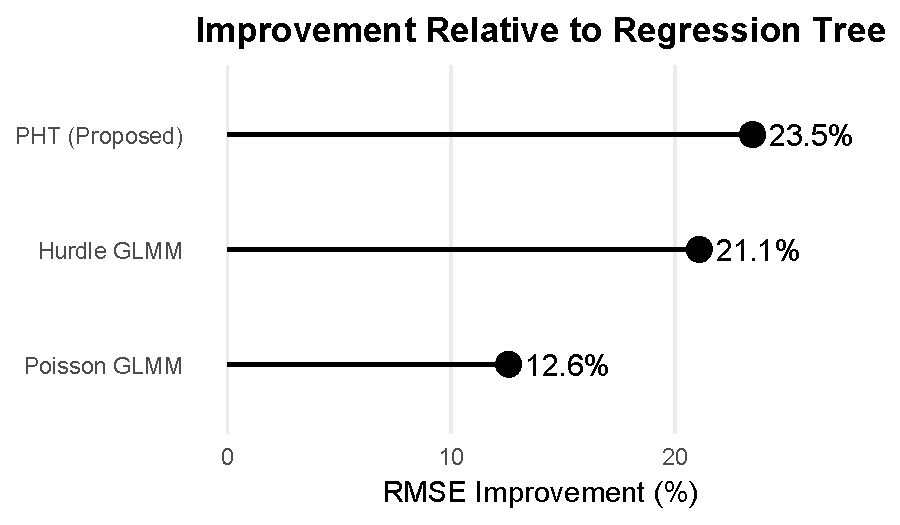
\includegraphics[width=0.4\textwidth]{Images/improvement.pdf}
		\caption{\footnotesize{Percentage reduction in RMSE relative to the standard Regression Tree}}
		\label{fig:improvement}
	\end{center}
\end{figure}
\section{Application to Real-World Ecological Data}
We demonstrate the proposed PHT algorithm on the \texttt{Salamanders} dataset
from the \texttt{glmmTMB} R package \citep{Brooks2017}, which records stream
salamander abundance at sites subject to mountaintop removal mining. The dataset
contains 644 observations across 23 sites, with seven salamander species
(\texttt{spp}), binary mining indicator (\texttt{mined}), percentage canopy
cover (\texttt{cover}), day of year (\texttt{DOY}), water temperature
(\texttt{Wtemp}), and days post-precipitation (\texttt{DOP}) as covariates.
Approximately 66\% of the count responses are zero, making this a canonical
setting for hurdle-type models. To obtain an honest assessment of out-of-sample predictive performance, we
partitioned the data at the \emph{site level}: 80\% of sites were assigned to
the training set and the remaining 20\% to the held-out test set.
This ensures that no observation from a test site appears during training,
thereby preventing information leakage arising from the longitudinal structure
of the data. PHT was compared against three benchmarks Regression Tree (A single CART tree fitted via
\texttt{rpart}, serving as the non-parametric baseline), Poisson GLMM (A generalised linear mixed model with a Poisson family and site-level random intercept, fitted with
\texttt{lme4}), and Hurdle GLMM (A hurdle model combining a zero/non-zero
Bernoulli component with a truncated-Poisson count component, both
with site-level random intercepts, fitted via \texttt{glmmTMB}). All predictions on the test set were generated at the population level (random effects set to zero), ensuring a fair comparison for new sites. Table~\ref{tab:salamander_results} reports MSE, RMSE, and MAE on the held-out test sites.
\begin{table}[ht]
	\centering
	\caption{Out-of-sample predictive performance on the \texttt{Salamanders}
		test set (20\% of sites)}
	\label{tab:salamander_results}
	\begin{tabular}{lccc}
		\hline
		\textbf{Model} & \textbf{MSE} & \textbf{RMSE} & \textbf{MAE} \\
		\hline
		Regression Tree  & 14.793 & 3.846 & 2.363 \\
		Poisson GLMM     & 14.706 & 3.835 & 2.146 \\
		Hurdle GLMM      & 13.561 & 3.683 & 2.108 \\
		\textbf{PHT (Proposed)} & \textbf{13.206} & \textbf{3.634} & \textbf{2.059} \\
		\hline
	\end{tabular}
\end{table}
PHT achieves the lowest error across all three metrics. Relative to the
Hurdle GLMM---the strongest parametric competitor---PHT reduces MSE by
$2.6\%$, RMSE by $1.3\%$, and MAE by $2.3\%$. The improvement over the
Regression Tree is more pronounced: $10.7\%$, $5.5\%$, and $12.8\%$
reductions in MSE, RMSE, and MAE, respectively. Figure~\ref{fig:vip} displays the variable importance scores for the positive
count component of the final PHT tree, computed as the total reduction in
weighted squared error attributable to each splitting variable.
\begin{figure}[ht]
	\centering
	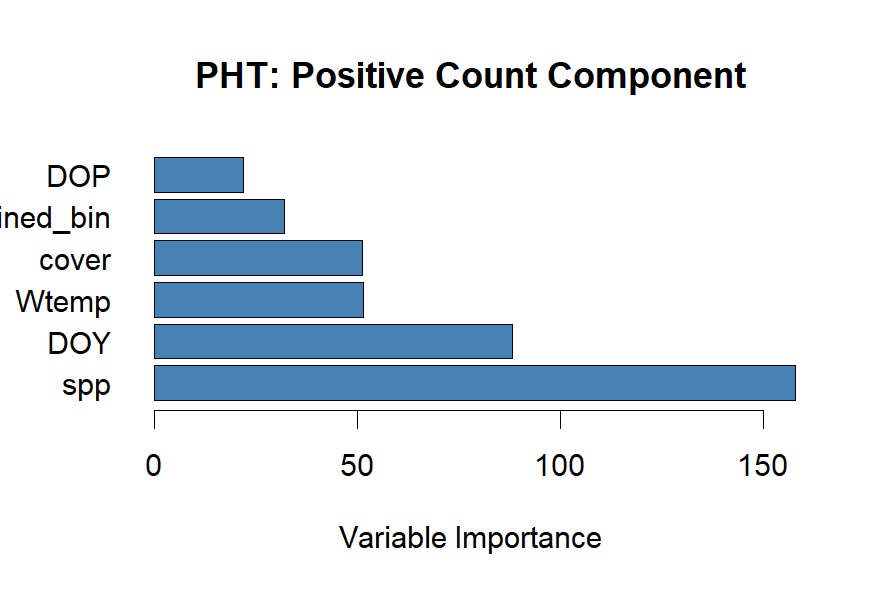
\includegraphics[width=0.6\linewidth]{Images/sam.png}
	\caption{Variable importance for the positive count component of PHT
		fitted to the \texttt{Salamanders} training data. Species
		identity (\texttt{spp}) and day of year (\texttt{DOY}) are
		the dominant drivers of non-zero salamander abundance.}
	\label{fig:vip}
\end{figure}
Species identity (\texttt{spp}) is by far the most influential predictor
($\text{importance} \approx 157$), followed by day of year (\texttt{DOY},
$\approx 87$), water temperature (\texttt{Wtemp}, $\approx 52$), and canopy
cover (\texttt{cover}, $\approx 51$). Mining status (\texttt{mined\_bin}) and
days post-precipitation (\texttt{DOP}) contribute comparatively less to the
positive count component. These findings are ecologically interpretable:
salamander abundance is strongly species-specific and exhibits clear seasonal
patterns, while habitat quality covariates play a secondary role.
\section{Future Work}
An important direction for future work is the construction of a unified hurdle-tree objective function that jointly incorporates both the zero and positive-count components during tree growth. Rather than estimating the two components separately, future versions of the algorithm may employ a global hurdle deviance or likelihood criterion for split selection, pruning, and convergence assessment. This could lead to stronger coupling between the two parts of the model and potentially yield improved predictive accuracy and interpretability.
\section*{Discussion and Conclusion}   
We introduced the PHT algorithm for longitudinal zero-inflated count data, which effectively captures nonlinear effects and within-subject dependence. Simulation and real-data analyses demonstrated its superior predictive accuracy over parametric and nonparametric benchmarks. Future work includes developing a unified likelihood-based splitting criterion.
%%%%%%%%%%%%%%%%%%%%%%%% References %%%%%%%%%%%%%%%%%%%%%%%%%%%%%
\begin{thebibliography}{9}
\bibitem[Brooks et al.(2017)]{Brooks2017}
Brooks, M.~E., Kristensen, K., van Benthem, K.~J., Magnusson, A., Berg, C.~W.,
Nielsen, A., Skaug, H.~J., M\"{a}chler, M. and Bolker, B.~M. (2017).
\newblock {glmmTMB} balances speed and flexibility among packages for
zero-inflated generalized linear mixed modeling.
\newblock {\it The R Journal}, 9(2), 378--400.

\bibitem[Hajjem et al. (2017)]{HLB17}
Hajjem A., Larocque D. and Bellavance F. (2017),
Generalized mixed effects regression trees,
{\it Statistics \& Probability Letters}, 126, 114--118.

\bibitem[McCulloch et al. (2008)]{MSN2008}
McCulloch C.~E., Searle S.~R. and Neuhaus J.~M. (2008),
{\it Generalized, Linear, and Mixed Models} (2nd ed.),
Hoboken, NJ: John Wiley \& Sons.

\bibitem[Min and Agresti (2005)]{MinAgresti2005}
Min Y. and Agresti A. (2005),
Random effects models for repeated measures of zero-inflated count data,
{\it Statistical Modelling}, 5(1), 1--19.

\bibitem[Sela and Simonoff (2012)]{sela2012re}
Sela R.~J. and Simonoff J.~S. (2012), 
RE-EM trees: A data mining approach for longitudinal and clustered data, 
{\it Machine Learning}, 86(2), 169--207.


\end{thebibliography}
 \end{document}

